\documentclass[11pt]{beamer}
\usetheme{Madrid}
\usepackage[utf8]{inputenc}

\usepackage{hyperref}
\usepackage{amsmath}
\usepackage{amsfonts}
\usepackage{amssymb}
\usepackage{graphicx}
\usepackage{algorithmic}
\usepackage{algorithm}
\usepackage{wrapfig}
\usepackage{subcaption}
\graphicspath{{.}}

% \setbeamercovered{transparent}
\title[Catalyst Acceleration]{Catalyst Meta Acceleration Framework: The history and the gist of it}
\author{Hongda Li}
\newcommand{\email}{alto@mail.ubc.ca}
\setbeamertemplate{navigation symbols}{}
\institute[]{UBC Okanagan}
\date{\today}
\subject{MATH 590 2024 Fall Winter}
\logo{}

% ---------------------------------------------------------
% Selecione um estilo de referência
\bibliographystyle{siam}

%\bibliographystyle{abbrv}
%\setbeamertemplate{bibliography item}{\insertbiblabel}
% ---------------------------------------------------------

% ---------------------------------------------------------
\newtheorem{remark}{Remark}
\newtheorem{assumption}{Assumption}
\usepackage{multicol}


% These are Heniz's notations. 
\newcommand{\To}{\ensuremath{\rightrightarrows}}
\newcommand{\GX}{\ensuremath{\Gamma}}
\newcommand{\mal}{\ensuremath{\mathfrak{m}}}
\newcommand{\mumu}{\ensuremath{{\mu\mu}}}
\newcommand{\paver}{\ensuremath{\mathcal{P}}}
\newcommand{\ZZZ}{\ensuremath{{X \times X^*}}}
\newcommand{\RRR}{\ensuremath{{\RR \times \RR}}}
\newcommand{\todo}{\hookrightarrow\textsf{TO DO:}}

\newcommand{\emp}{\ensuremath{\varnothing}}
%\newcommand{\la}{\ensuremath{\langle}}
%\newcommand{\ra}{\ensuremath{\rangle}}
\newcommand{\infconv}{\ensuremath{\mbox{\small$\,\square\,$}}}
\newcommand{\pscal}{\ensuremath{\scal{\cdot}{\cdot}}}
\newcommand{\Tt}{\ensuremath{\mathfrak{T}}}
\newcommand{\YY}{\ensuremath{\mathcal Y}}
\newcommand{\XX}{\ensuremath{\mathcal X}}
\newcommand{\HH}{\ensuremath{\mathcal H}}
\newcommand{\XP}{\ensuremath{\mathcal X}^*}
\newcommand{\st}{\ensuremath{\;|\;}}
\newcommand{\zeroun}{\ensuremath{\left]0,1\right[}}

\newcommand{\lev}[1]{\ensuremath{\mathrm{lev}_{\leq #1}\:}}
\newcommand{\moyo}[2]{\ensuremath{\sideset{_{#2}}{}{\operatorname{}}\!#1}}
\newcommand{\pair}[2]{\left\langle{{#1},{#2}}\right\rangle}
%\newcommand{\scal}[2]{\left.\left\langle{#1}\:\right| {#2}  \right\rangle}
\newcommand{\scal}[2]{\langle{{#1},{#2}}\rangle}
\newcommand{\Scal}[2]{\left\langle{{#1},{#2}}\right\rangle}
%\newcommand{\scal}[2]{\braket{ {#1},{#2}}}

\newcommand{\yosida}{\ensuremath{ \; {}^}}
\newcommand{\exi}{\ensuremath{\exists\,}}
\newcommand{\GG}{\ensuremath{\mathcal G}}
\newcommand{\RR}{\ensuremath{\mathbb R}}
\newcommand{\SSS}{\ensuremath{\mathbb S}}
\newcommand{\CC}{\ensuremath{\mathbb C}}
\newcommand{\Real}{\ensuremath{\mathrm{Re}\,}}
\newcommand{\ii}{\ensuremath{\mathrm i}}
\newcommand{\RP}{\ensuremath{\left[0,+\infty\right[}}
\newcommand{\RPX}{\ensuremath{\left[0,+\infty\right]}}
\newcommand{\RPP}{\ensuremath{\,\left]0,+\infty\right[}}
\newcommand{\RX}{\ensuremath{\,\left]-\infty,+\infty\right]}}
\newcommand{\RXX}{\ensuremath{\,\left[-\infty,+\infty\right]}}
\newcommand{\KK}{\ensuremath{\mathbb K}}
\newcommand{\NN}{\ensuremath{\mathbb N}}
\newcommand{\nnn}{\ensuremath{{n \in \NN}}}
\newcommand{\thalb}{\ensuremath{\tfrac{1}{2}}}
\newcommand{\zo}{\ensuremath{{\left]0,1\right]}}}
\newcommand{\lzo}{\ensuremath{{\lambda \in \left]0,1\right]}}}
%\newcommand{\toppsepp}{\setlength{\partopsep}{-5pt}}
\newcommand{\menge}[2]{\big\{{#1} \mid {#2}\big\}}
\newcommand{\pfrac}[2]{\ensuremath{\mathlarger{\tfrac{#1}{#2}}}}


% MATH OPERATORS ===============================================================
% \newcommand{\monos}{\ensuremath{\mathcal M}}
\newcommand{\DD}{\operatorname{dom}f}
\newcommand{\IDD}{\ensuremath{\operatorname{int}\operatorname{dom}f}}
\newcommand{\CDD}{\ensuremath{\overline{\operatorname{dom}}\,f}}
\newcommand{\clspan}{\ensuremath{\overline{\operatorname{span}}}}
\newcommand{\cone}{\ensuremath{\operatorname{cone}}}
\newcommand{\dom}{\ensuremath{\operatorname{dom}}}
\newcommand{\closu}{\ensuremath{\operatorname{cl}}}
\newcommand{\cont}{\ensuremath{\operatorname{cont}}}
\newcommand{\mons}{\ensuremath{\mathcal{A}}}
\newcommand{\gra}{\ensuremath{\operatorname{gra}}}
\newcommand{\epi}{\ensuremath{\operatorname{epi}}}
\newcommand{\prox}{\ensuremath{\operatorname{Prox}_{\mu}}}
\newcommand{\hprox}{\ensuremath{\operatorname{prox}}}
\newcommand{\intdom}{\ensuremath{\operatorname{int}\operatorname{dom}}\,}
\newcommand{\inte}{\ensuremath{\operatorname{int}}}
\newcommand{\sri}{\ensuremath{\operatorname{sri}}}
\newcommand{\reli}{\ensuremath{\operatorname{ri}}}
\newcommand{\cart}{\ensuremath{\mbox{\LARGE{$\times$}}}}


\newcommand{\average}{\ensuremath{\mathcal{R}_{\mu}({\bf A},{\boldsymbol \lambda})}}
\newcommand{\averagebar}{\ensuremath{\mathcal{R}_{1}({\bf A},\bar{\lambda})}}
\newcommand{\averageonelambda}{\ensuremath{\mathcal{R}({\bf A},{\boldsymbol \lambda})}}
\newcommand{\averageonehalf}{\ensuremath{\mathcal{R}_{1}(A,1/2)}}
\newcommand{\averageinverse}{\ensuremath{\mathcal{R}_{\mu^{-1}}({\bf A}^{-1},{\boldsymbol \lambda})}}
\newcommand{\averageoneinverse}{\ensuremath{\mathcal{R}({\bf A}^{-1},{\boldsymbol \lambda})}}
\newcommand{\averagef}{\ensuremath{\mathcal{P}_{\mu}(f,\lambda)}}
\newcommand{\averagefone}{\ensuremath{\mathcal{P}_{1}(f,\lambda)}}
\newcommand{\averagefd}{\ensuremath{\mathcal{P}_{\mu}((f_{1},\ldots, f_{n}),(\lambda_{1},\ldots, \lambda_{n}))}}
\newcommand{\averagefik}{\ensuremath{\mathcal{P}_{\mu_{k}}((f_{1,k},\ldots,f_{n,k}),
(\lambda_{1,k},\ldots,\lambda_{n,k}))}}
\newcommand{\averagesub}{\ensuremath{\mathcal{R}_{\mu}(\partial f,\lambda)}}
\newcommand{\res}{\ensuremath{\mathcal{R}_{\mu}}}
\newcommand{\resmuk}{\ensuremath{\mathcal{R}_{\mu_{k}}}}
\newcommand{\newres}{\ensuremath{\mathcal{R}}}
\newcommand{\resmualpha}{\ensuremath{\mathcal{R}_{\alpha\mu}}}
\newcommand{\averageone}{\ensuremath{\mathcal{R}_{1}}}
\newcommand{\harm}{\ensuremath{\mathcal{H}(A,\lambda)}}
\newcommand{\arithmetic}{\ensuremath{\mathcal{A}(A,\lambda)}}

\newcommand{\WC}{\ensuremath{{\mathfrak W}}}
\newcommand{\SC}{\ensuremath{{\mathfrak S}}}
\newcommand{\card}{\ensuremath{\operatorname{card}}}
\newcommand{\bd}{\ensuremath{\operatorname{bdry}}}
\newcommand{\ran}{\ensuremath{\operatorname{ran}}}
\newcommand{\rec}{\ensuremath{\operatorname{rec}}}
\newcommand{\rank}{\ensuremath{\operatorname{rank}}}
\newcommand{\kernel}{\ensuremath{\operatorname{ker}}}
\newcommand{\conv}{\ensuremath{\operatorname{conv}}}
\newcommand{\segh}{\ensuremath{\operatorname{seg}}}
\newcommand{\boxx}{\ensuremath{\operatorname{box}}}
\newcommand{\clconv}{\ensuremath{\overline{\operatorname{conv}}\,}}
\newcommand{\cldom}{\ensuremath{\overline{\operatorname{dom}}\,}}
\newcommand{\clran}{\ensuremath{\overline{\operatorname{ran}}\,}}
\newcommand{\Nf}{\ensuremath{\nabla f}}
\newcommand{\NNf}{\ensuremath{\nabla^2f}}
\newcommand{\Fix}{\ensuremath{\operatorname{Fix}}}
\newcommand{\FFix}{\ensuremath{\overline{\operatorname{Fix}}\,}}
\newcommand{\aFix}{\ensuremath{\widetilde{\operatorname{Fix}\,}}}
\newcommand{\Id}{\ensuremath{\operatorname{Id}}}
\newcommand{\Max}{\ensuremath{\operatorname{max}}}
\newcommand{\Bb}{\ensuremath{\mathfrak{B}}}
\newcommand{\BB}{\ensuremath{\mathbb{B}}}
\newcommand{\Fb}{\ensuremath{\overrightarrow{\mathfrak{B}}}}
\newcommand{\Fprox}{\ensuremath{\overrightarrow{\operatorname{prox}}}}
\newcommand{\Bprox}{\ensuremath{\overleftarrow{\operatorname{prox}}}}
\newcommand{\Bproj}{\ensuremath{\overleftarrow{\operatorname{P}}}}
\newcommand{\Ri}{\ensuremath{\mathfrak{R}_i}}
\newcommand{\Dn}{\ensuremath{\,\overset{D}{\rightarrow}\,}}
\newcommand{\nDn}{\ensuremath{\,\overset{D}{\not\rightarrow}\,}}
\newcommand{\weakly}{\ensuremath{\,\rightharpoonup}\,}
\newcommand{\weaklys}{\ensuremath{\,\overset{*}{\rightharpoonup}}\,}
\newcommand{\gr}{\ensuremath{\operatorname{gra}}}
\newcommand{\g}{\ensuremath{\,\overset{g}{\rightarrow}}\,}
\newcommand{\p}{\ensuremath{\,\overset{p}{\rightarrow}}\,}
\newcommand{\e}{\ensuremath{\,\overset{e}{\rightarrow}}\,}
\newcommand{\Tbar}{\ensuremath{\overline{T}}}
\newcommand{\n}{\ensuremath{\,\overset{n}{\rightarrow}}\,}

\newcommand{\minf}{\ensuremath{-\infty}}
\newcommand{\pinf}{\ensuremath{+\infty}}
\renewcommand{\iff}{\ensuremath{\Leftrightarrow}}
% \renewcommand{\phi}{\ensuremath{\varphi}}
%\newcommand{\Real}{\ensuremath{\mathrm{Re}\,}}
\newcommand{\negent}{\ensuremath{\operatorname{negent}}}
\newcommand{\neglog}{\ensuremath{\operatorname{neglog}}}
\newcommand{\halb}{\ensuremath{\tfrac{1}{2}}}
\newcommand{\bT}{\ensuremath{\mathbf{T}}}
\newcommand{\bX}{\ensuremath{\mathbf{X}}}
\newcommand{\bL}{\ensuremath{\mathbf{L}}}
\newcommand{\bD}{\ensuremath{\boldsymbol{\Delta}}}
\newcommand{\bc}{\ensuremath{\mathbf{c}}}
\newcommand{\by}{\ensuremath{\mathbf{y}}}
\newcommand{\bx}{\ensuremath{\mathbf{x}}}
\newcommand{\bA}{{\bf A}}
\newcommand{\Other}{Indeterminate }
\newcommand{\other}{indeterminate }


%%% Raf's stuff  ===============================================================
\newcommand{\al}{\alpha}
\newcommand{\la}{\lambda}
\newcommand{\La}{\Lambda}
\newcommand{\pluss}{{\hskip1pt \raise1pt\vbox{\hrule width6pt \vskip1pt
\hrule width6pt}\kern-4pt{\lower1pt\hbox{\vrule height6pt \kern1pt\vrule
height6pt}}\hskip5pt}}
\newcommand{\timess}{\star}
\newcommand{\argmax}{\mathop{\rm argmax}\limits}
\newcommand{\argmin}{\mathop{\rm argmin}\limits}
\newcommand{\product}{\langle\cdot,\cdot\rangle}
\newcommand{\im}{\mathrm{Im}}
\newcommand{\multival}{\ensuremath{X\to 2^{X^*}}}
\newcommand{\SX}{\ensuremath{2^{X^*}}}
% proof with breaks
\usepackage[most]{tcolorbox}
% \useinnertheme{tcolorbox}
\tcbset{breakable,title after break=\insertblocktitle}



\begin{document}

\begin{frame}
    \titlepage
\end{frame}

\begin{frame}{ToC}
    \begin{multicols}{2}
        \tableofcontents
    \end{multicols}
\end{frame}

%     \subsection{Taxonomy of Proximal type of Methods}
%         \begin{frame}{Frame Title}
%             \begin{block}{Formula Presented in Block}
%                 \begin{align}
%                     \min_{x} g(x) + h(x)
%                 \end{align}    
%             \end{block}
%             \begin{itemize}
%                 \item [1.]Throughout this presentation, we assume the objective of a function $f$ is the sum of 2 functions.
%                 \item [2.]We are interested in the paper: FISTA (Fast Iterative-Shrinkage Algorithm) by Beck and Teboulle \cite{paper:FISTA}. 
%                 \pause 
%                 \item [1.] When $h = \delta_Q$ with $Q$ closed and convex with $Q\subseteq \text{ri}\circ \text{dom}(g)$, we use projected subgradient. 
%                 \item [2.] When $g$ is \textbf{\emph{strongly smooth}} and $h$ is \textbf{closed convex proper} whose proximal oracle is easy to compute, we consider the use of FISTA. 
%             \end{itemize}           
%         \end{frame}    
%     \subsection{The Proximal Operator}
%         \begin{frame}{Frame Title}
%             \begin{definition}[Definition of Something]
%                 Let $f$ be convex closed and proper, then the proximal operator parameterized by $\alpha > 0$ is a non-expansive mapping defined as: 
%                 \begin{align*}
%                     \text{prox}_{f, \alpha}(x) := 
%                     \arg\min_{y}\left\lbrace
%                         f(y) + \frac{1}{2\alpha} \Vert y - x\Vert^2
%                     \right\rbrace. 
%                 \end{align*}
%             \end{definition}  
%             \begin{remark}
%                 When $f$ is convex, closed, and proper, 
%             \end{remark}
%         \end{frame}
%         \begin{frame}{Prox is the Resolvant of Subgradient}
%             \begin{lemma}[The Lemma]\label{lemma:prox_alternative_form}
%                 When the function $f$ is convex closed and proper, the $\text{prox}_{\alpha, f}$ can be viewed as the following operator $(I + \alpha \partial f)^{-1}$. 
%             \end{lemma}
%             \begin{proof}
%                 Minimizer satisfies zero subgradient condition, 
%                 {\scriptsize
%                 \begin{align*}
%                     \mathbf 0 &\in \partial
%                     \left[
%                         \left.
%                             f(y) + \frac{1}{2\alpha} \Vert y - x\Vert^2 
%                         \right| y
%                     \right](y^+)
%                     \\
%                     \mathbf 0 &\in \partial f(y^+) + \frac{1}{\alpha}(y^+ - x)
%                     \\
%                     \frac{x}{\alpha} &\in 
%                     (\partial f + \alpha^{-1}I)(y^+)
%                     \\
%                     x &\in 
%                     (\alpha \partial f + I)(y^+)
%                     \\
%                     y &\in (\alpha\partial f+ I)^{-1}(x).
%                 \end{align*}
%                 }
%             \end{proof}
%         \end{frame}
        
%     \subsection{Strong Smoothness}
%         \begin{frame}{Equivalence of Strong Smoothness and Lipschitz Gradient}
%             \begin{theorem}[Lipschitz Gradient Equivalence under Convexity]
%                 Suppose $g$ is differentiable on the entire of $\mathbb E$. It is closed convex proper. It is strongly smooth with parameter $\alpha$ if and only if the gradient $\nabla g$ is globally Lipschitz continuous with a parameter of $\alpha$ and $g$ is closed and convex. 
%                 \begin{align*}
%                     \Vert \nabla g(x) -\nabla g(y)\Vert \le 
%                     \alpha 
%                     \Vert x - y \Vert\quad \forall x, y\in \mathbb E
%                 \end{align*}
%             \end{theorem}
%             \begin{proof}
%                 Using line integral, we can prove Lipschitz gradient implies strong smoothness without convexity. The converse requires convexity and applying generalized Cauchy Inequality to (iv) in Theorem 5.8 for Beck's textbook \cite{book:first_order_opt}. 
%             \end{proof}
%         \end{frame}
%     \subsection{A Major Assumption}    
%         \begin{frame}{A Major Assumption}
%             \begin{assumption}[Convex Smooth Nonsmooth with Bounded Minimizers]\label{assumption:1}
%                 We will assume that $g:\mathbb E\mapsto \mathbb R$ is \textbf{strongly smooth} with constant $L_g$ and $h:\mathbb E \mapsto \bar{\mathbb R}$ \textbf{is closed convex and proper}. We define $f := g + h$ to be the summed function and $\text{ri}\circ \text{dom}(g) \cap \text{ri}\circ \text{dom}(h) \neq \emptyset$. We also assume that a set of minimizers exists for the function $f$ and that the set is bounded. Denote the minimizer using $\bar x$. 
%             \end{assumption}
%         \end{frame}
        
    
% \section{A New Fancy Section}
%     \subsection{A Fancy Subsetction for Algorithm}
%         \begin{frame}{The Accelerated Proximal Gradient Method}
%             \begin{block}{Momentum Template Method}
%                 \begin{algorithm}[H]
%                     \begin{algorithmic}[1]
%                         \STATE{\textbf{Input:} $x^{(0)}, x^{(-1)}, L, h, g$; 2 initial guesses and stepsize L}
%                         \STATE{$y^{(0)} = x^{(0)} + \theta_k (x^{(0)} - x^{(-1)})$}
%                         \FOR{$k = 1, \cdots, N$}
%                             \STATE{$x^{(k)} = \text{prox}_{h, L^{-1}}(y^{(k)} + L^{-1}\nabla g(y^{(k)})) =: \mathcal P_{L^{-1}}^{g, h}(y^{(k)})$}
%                             \STATE{$y^{(k + 1)} = x^{(k)} + \theta_k(x^{(k)} - x^{(k - 1)})$}
%                         \ENDFOR
%                     \end{algorithmic}
%                     \caption{Template Proximal Gradient Method With Momentum}\label{alg:fista_template}
%                 \end{algorithm}
%             \end{block}
%         \end{frame}

\section{Introduction}
    \subsection{Major references}
        \begin{frame}{Nesterov's Book}
            \begin{figure}
                \centering
                
\includegraphics[width=10em]{assets/Nesterov Book.png}    
            \end{figure}
            \begin{itemize}
                \item Yurri Nesterov's book: ``Lectures on Convex Optimization'' 2018, Springer \cite{nesterov_lectures_2018}. 
            \end{itemize}
        \end{frame}
        \begin{frame}{Accelerated Proximal Point Method (PPM)}
            \begin{figure}
                \centering
                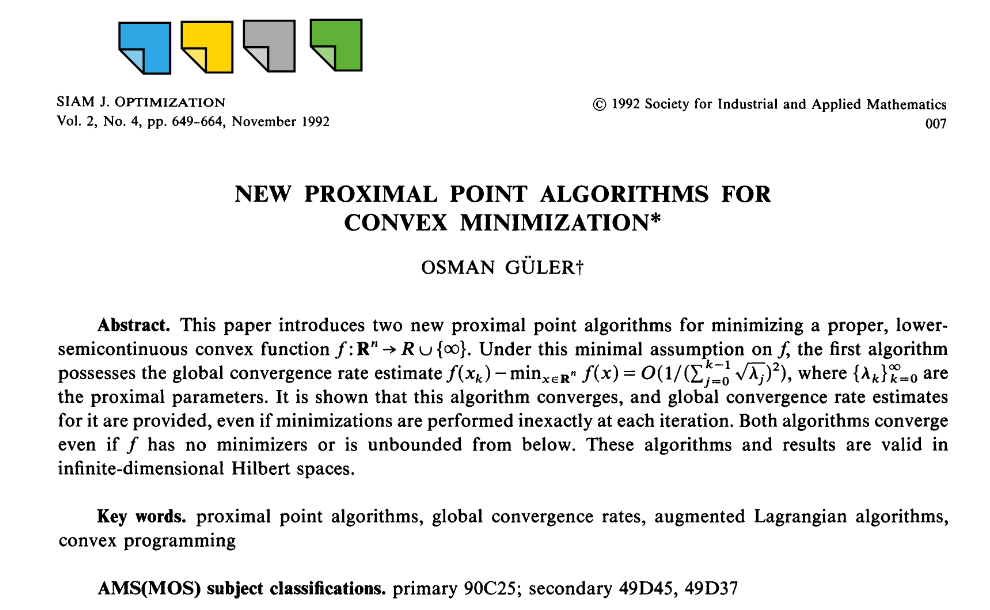
\includegraphics[width=25em]{assets/Acc ppm}
            \end{figure}
            \begin{itemize}
                \item Osman Guler's: ``New proximal point algorithm for convex optimization'', SIAM J. Optimization 1992 \cite{guler_new_1992}. 
            \end{itemize}
        \end{frame}
        \begin{frame}{Catalyst Acceleration}
            \begin{figure}
                \centering
                \subfloat[Lin 2015\label{fig:a}]{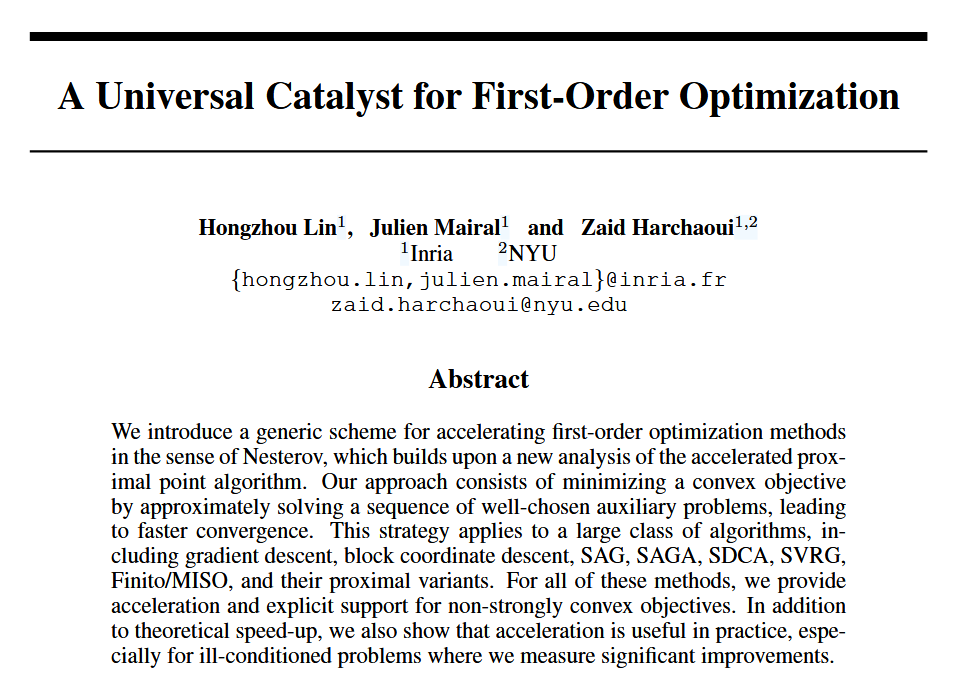
\includegraphics[width=15em]{assets/lin2015.png}}
                \subfloat[Paquette 2018\label{fig:b}]{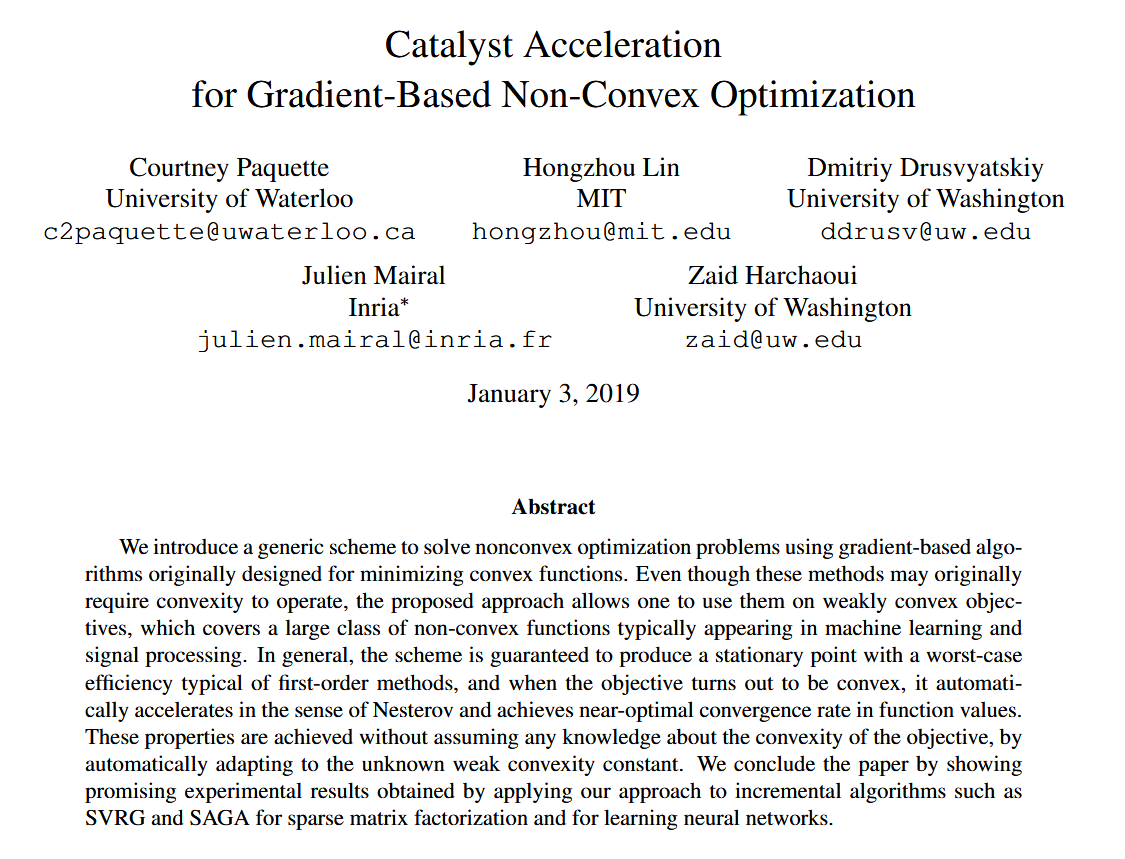
\includegraphics[width=15em]{assets/paquette 2018.png}}
                % \caption{Lin's }
                % \label{fig:1}
            \end{figure}
            \begin{itemize}
                \item Hongzhou Lin et al. ``Universal Catalyst for first order optimization'', 2015 NISP \cite{lin_universal_2015}.
                \item Paquette et al. ``Catalyst for gradient-based non-convex optimization'', 2018 JMLR \cite{paquette_catalyst_2018}. 
            \end{itemize}
        \end{frame}
        \begin{frame}{Objectives of the Talk}
            \begin{block}{List of objectives}
                \begin{enumerate}
                    \item Introduce the technique of Nesterov's estimating sequence. 
                    \item Survey the history of the Catalyst algorithm (Catalyst for short).  
                    \item Survey the theories behind Catalyst. 
                    \item Highlight key innovations. 
                    \item Introduce the non-convex extension of Catalyst. 
                \end{enumerate}
            \end{block}
            \pause
            \begin{block}{A note on the scope}
                Specific applications and algorithms are outside the scope because variance reduced stochastic method is itself a big topic.     
            \end{block}
        \end{frame}

    \subsection{Nesterov's Estimating Sequence}
        \begin{frame}{Nesterov's Estimating Sequence}            
            \begin{definition}[Nesterov's estimating sequence]\label{def:nes-est-seq}
                Let $(\phi_k : \RR^n \rightarrow \RR)_{k \ge 0}$ be a sequence of functions. 
                It's an estimating sequence when it satisfies the conditions: 
                \begin{enumerate}
                    \item $\exists (x_k)_{k \ge 0}$ such that for all $k \ge 0$ it has $F(x_k) \le \phi_k^*: =\min_{x}\phi_k(x)$. 
                    \item $\exists (\alpha_k)_{k \ge 0}$ where $\alpha_k \in (0, 1)$ such that $\phi_{k + 1}(x) - \phi_k(x) \le - \alpha_k(\phi_k(x) - F(x))$ for all $k\ge 0, x \in \RR^n$.
                \end{enumerate}
            \end{definition}
        \end{frame}

        \begin{frame}{Nesterov's Estimating Sequence and Convergence}
            \begin{block}{Observations}
                {\small
                If we define $\Delta_k(x) := \phi_k (x) - F(x)$ for all $x \in \RR^n$, assume that $F$ has minimizer $x^*$. 
                Then $\forall k \ge 0$:  
                \begin{align*}
                    \phi_{k + 1}(x) - \phi_k(x) 
                    &\le - \alpha_k (\phi_k(x) - F(x))
                    \\
                    \iff 
                    \phi_{k + 1}(x) - F(x) - (\phi_k(x) - F(x))
                    &\le 
                    -\alpha_k(\phi_k(x) - F(x))
                    \\
                    \iff
                    \Delta_{k + 1}(x) - \Delta_k(x) &\le
                    - \alpha_k\Delta_k(x)
                    \\
                    \iff 
                    \Delta_{k + 1}(x) 
                    &\le 
                    (1 - \alpha_k)\Delta_k(x). 
                \end{align*}
                Unroll the recurrence, by setting $x = x^*$, $\Delta_k(x^*)$ is non-negative. By the properties of Nesterov's estimating: 
                \begin{align*}
                    0\le F(x_k) - F(x^*) \le \phi_k^* - F(x^*) \le \Delta_k(x^*) 
                    &= \phi_k(x^*) - F(x^*) 
                    \\
                    &\le \left(\prod_{i = 0}^k(1 - \alpha_i)\right)\Delta_0(x^*).
                \end{align*}
                }
            \end{block}
        \end{frame}

    \subsection{Example: Accelerated Proximal Gradient}
        \begin{frame}{Example: Accelerated Proximal Gradient}
            The following algorithm is proved in the report which it's similar to Nesterov's 2.2.20 in his book \cite{nesterov_lectures_2018}. 
            \begin{block}{Quick Notations}
                Assume $F = f + g$ where $f$ is $L$-Lipschitz smooth and $\mu \ge 0$ strongly convex and $g$ is convex. 
                Define
                \begin{align*}
                    \mathcal M^{L^{-1}}(x; y) 
                    &:= g(x) + f(y) 
                    + 
                    \left\langle \nabla f(y), x - y\right\rangle 
                    + 
                    \frac{L}{2}\Vert x - y\Vert^2, 
                    \\
                    \widetilde{\mathcal J}_{L^{-1}}y 
                    &:= \argmin_{x} \mathcal M^{L^{-1}}(x; y), 
                    \\
                    \mathcal G_{L^{-1}}(y)
                    &:= L\left(I - \widetilde{\mathcal J}_{L^{-1}}\right)y. 
                \end{align*}
            \end{block}
        \end{frame}
        \begin{frame}{Example: Accelerated Proximal Gradient}
            \begin{definition}[estimating sequence for Accelerated Proximal Gradient]
                \label{def:nes-est-seq-pg}
                {\small
                    $(\phi_k)_{k \ge0}$ is the Nesterov's estimating sequence recursively given by: 
                    \begin{align*}
                        &\textcolor{red}{
                            l_F(x; y_k) := 
                            F\left(\widetilde{\mathcal J}_{L^{-1}} y_k \right) 
                            + \langle \mathcal G_{L^{-1}}y_k, x - y_k\rangle + 
                            \frac{1}{2L}\Vert \mathcal G_{L^{-1}}y_k\Vert^2,
                        } 
                        \\
                        & 
                        \phi_{k + 1}(x)
                        := (1 - \alpha_k)\phi_k (x) + 
                        \alpha_k 
                        \left(
                            l_F(x; y_k) + \frac{\mu}{2}\Vert x - y_k\Vert^2
                        \right). 
                    \end{align*}
                    The Algorithm generates a sequence of vectors $y_k, x_k$, and scalars $\alpha_k$ satisfies the following: 
                    \begin{align*}
                        &x_{k + 1} = \widetilde{\mathcal J}_{L^{-1}} y_k, 
                        \\
                        & \text{find } \alpha_{k + 1} \in (0, 1): 
                        \alpha_{k + 1} = (1 - \alpha_{k + 1})\alpha_k^{2} + (\mu/L) \alpha_{k + 1}
                        \\
                        &y_{k + 1} = x_{k + 1} + \frac{\alpha_k(1 - \alpha_k)}{\alpha_k^2 + \alpha_{k + 1}}(x_{k + 1} - x_k). 
                    \end{align*}
                    One of the possible base case can be $x_0 = y_0$ and any $\alpha_0 \in (0, 1)$. 
                }
            \end{definition}
        \end{frame}

\section{Guler 1992}
    \begin{frame}{Guler 1992: Accelerated Proximal Point Method}
        Guler in 1992 discovered the following: 
        \begin{enumerate}
            \item The method of proximal point can be accelerated via Nesterov's estimating sequence. 
            \item The accelerated convergence rate retains for certain magnitude of errors on inexact evaluation of proximal point method. 
        \end{enumerate}
        \begin{block}{Quick notations}
            We use the following list of notations: 
            \begin{align*}
                \mathcal M^{\lambda} (x; y) &:= F(x) + \frac{1}{2\lambda}\Vert x - y\Vert^2
                \\
                \mathcal J_\lambda y &:= \argmin_x \mathcal M^{\lambda} (x; y)
                \\
                \mathcal G_\lambda &:= \lambda^{-1}(I - \mathcal J_\lambda). 
            \end{align*}
            We use $\mathcal G_k, \mathcal J_k, \mathcal M_k$ as a short for $\mathcal G_{\lambda_k}, \mathcal J_{\lambda_k}, \mathcal M_{\lambda_k}$. 
            $(\lambda_k)_{k \ge0}$ is a sequence that controls proximal operator. 
        \end{block}
    \end{frame}
    \subsection{Exact accelerated PPM}
        \begin{frame}{Estimating sequence of accelerated PPM}
            \begin{definition}[Accelerated PPM estimating sequence]
                {\small
                    \label{def:nes-est-seq-acc-ppm}
                    $(\phi_k)_{k \ge0}$ has for all $k \ge0$, any $A \ge 0$: 
                    \begin{align*}
                        \phi_0 &:= f(x_0) + \frac{A}{2}\Vert x - x_0\Vert^2, 
                        \\
                        \phi_{k + 1}(x) &:= 
                        (1 - \alpha_k)\phi_k(x)
                        + 
                        \alpha_k(
                            \textcolor{red}
                            {
                                F(\mathcal J_k y_k) + \langle \mathcal G_k y_k, x - \mathcal J_k y_k\rangle
                            }
                        ).    
                    \end{align*}
                    $(\lambda_k)_{k \ge 0}$, $x_k = \mathcal J_\lambda y_k$. 
                    Auxiliary vectors $(y_k, v_k)$, and $(\alpha_k, A_k)_{k\ge 0}$ satisfies $k\ge0$:
                    \begin{align*}
                        \alpha_k &= \frac{1}{2}\left(
                            \sqrt{(A_k\lambda_k)^2 + 4A_k \lambda_k}
                            - A_k\lambda_k
                        \right), 
                        \\
                        y_k &= (1 - \alpha_k)x_k + \alpha_k v_k, 
                        \\
                        v_{k + 1}
                        &= 
                        v_k - \frac{\alpha_k}{A_{k + 1}\lambda_k}(y_k - \mathcal J_k y_k), 
                        \\
                        A_{k + 1} &= (1 - \alpha_k)A_k. 
                    \end{align*}
                }
            \end{definition}
        \end{frame}
        \begin{frame}{Convergence of accelerated PPM} 
            We now state a major result of Guler 1992 \cite{guler_new_1992} on accelerated PPM. 
            \begin{block}{Accelerated rate of convergence from Guler}
                The accelerated PPM generate $(x_k)_{k\ge 0}$ such that $F(x_k) - F^*$ converges at a rate of: 
                {\large
                \begin{align*}
                    \mathcal O\left(
                        \frac{1}{\left(
                            \sum_{i = 1}^{k}\sqrt{\lambda_i}
                        \right)^2}
                    \right). 
                \end{align*}    
                }
            \end{block}
            Note, PPM without accelerate converges at a rate of $\mathcal O((\sum_{i = 1}^{k}\lambda_i)^{-1})$, this is from Guler too. 
        \end{frame}
    \subsection{Inexact accelerated PPM}
        \begin{frame}{Accelerated Inexact PPM}
            Guler cited Rockafellar 1976 \cite{rockafellar_monotone_1976} for condition (A'): 
            \begin{align*}
                x_{k + 1}\approx \mathcal J_{k} y_k \text{ be such that: }
                \dist\left(
                    \mathbf 0, \partial \mathcal M^{k}(x_{k + 1}; y_k)
                \right) &\le \frac{\epsilon_k}{k}
                \\
                \implies 
                \Vert x_{k + 1} - \mathcal J_{k}y_k\Vert 
                &\le \epsilon_k. 
            \end{align*}
            Putting things into the context of accelerated PPM, the theorem follows is pivotal: 
            \begin{theorem}[\small Guler's inexact proximal point error bound (Lemma 3.1)]
                Define Moreau Envelope at $y_k$: $\mathcal M_k^* := \min_z \mathcal {M}^{\lambda_k}(z; y_k)$. 
                If $x_{k +1}$ is an inexact evaluation under condition (A'), then: 
                \begin{align*}
                    \frac{1}{2\lambda_k} \Vert x_{k + 1} - \mathcal J_k y_k\Vert^2
                    &\le 
                    \mathcal M_k(x_{k + 1}, y_k) - \mathcal M^*_k
                    \le \frac{\epsilon_k^2}{2\lambda_k}. 
                \end{align*}
            \end{theorem}
        \end{frame}
        \begin{frame}{Guler's Major Results}
            The following is a major result from Guler \cite{guler_new_1992} on inexact accelerated PPM. 
            \begin{theorem}[\small Guler's accelerated inexact PPM convergence (Theorem 3.3)]
                If the error sequence $(\epsilon_k)_{k \ge0}$ for condition A' is bounded by $\mathcal O(1/k^\sigma)$ for some $\sigma > 1/2$, then the accelerated proximal point method has for any feasible $x \in \RR^n$: 
                \begin{align*}
                    f(x_k) - f(x) \le \mathcal O(1/k^2) + \mathcal (1 / k^{2\sigma - 1}) \rightarrow 0. 
                \end{align*}    
            \end{theorem}
            If $\sigma \ge 3/2$, the method converges at a rate of $\mathcal O(1/k^2)$. 
            \pause 
            It looks exciting, but it's not exciting for practical purposes because: 
            \begin{enumerate}
                \item Determining $(\epsilon_k)_{k\ge 0}$ requires knowledge on $\phi_k^*$. 
                \item $\phi_k^*$ is expressed with intractable quantity: $F(\mathcal J_k y_k)$. 
            \end{enumerate}
            So the algorithm contains intractable quantities: $F(\mathcal J_k y_k)$. 
            \textcolor{red}{It's not yet ready to be formulated into a concrete algorithm.}
        \end{frame}
\section{Lin 2015}
    \begin{frame}{Lin 2015}
        Hongzhou Lin 2015 \cite{lin_universal_2015} did the following: 
        {\small
        \begin{enumerate}
            \item Improved the proof from Guler 1992 to include strongly convex objectives. 
            \item Showed that $(\epsilon_k)_{k\ge 0}$ can be determined algorithmically and  an accelerated rate can be achieved. 
            \item Invented his own accelerated variance reduced incremental method called: ``Accelerated MISO-Prox" to demonstrate the Catalyst Framework. 
            \item First time in history he obtained an accelerated rate for incremental methods in general. 
        \end{enumerate}
        }
        \begin{block}{Quick notations}
            Assume $F$ is a $\mu \ge 0$ strongly convex function. 
            Fix $\kappa$ and the notations are: 
            \begin{align*}
                \mathcal M^{\kappa^{-1}}(x; y) &:= F(x) + \frac{\kappa}{2}\Vert x - y\Vert^2, 
                \\
                \mathcal J_{\kappa^{-1}} y &:= \argmin_x \mathcal M^{\kappa^{-1}} (x, y). 
            \end{align*}
        \end{block}
    \end{frame}
    \subsection{The Catalyst Algorithm}
        \subsection{The algorithm}
            \begin{frame}{Lin's accelerated proximal point method}
                \begin{definition}[Lin's accelerated proximal point method]
                    Initialize any $y_0 = x_0 \in \RR^n$, fix parameters $\kappa$ and $\alpha_0$. 
                    Let $(\epsilon_k)_{k \ge 0}$ be the error of inexact proximal point evaluations. 
                    Then the algorithm generates $(x_k, y_k)$ satisfies for all $k \ge 1$: 
                    {\small
                    \begin{align*}
                        & \text{find } x_k \approx \mathcal J_{\kappa^{-1}} y_{k - 1} \text{ such that } \mathcal M^{\kappa^{-1}}(x_k, y_{k - 1}) - \mathcal M^{\kappa^{-1}}(\mathcal J_{\kappa^{-1}}y_{k - 1}, y_{k - 1}) \le \epsilon_k
                        \\
                        & \text{find } \alpha_k \in (0, 1) \text{ such that } \alpha_k^2 = (1 - \alpha_k)\alpha_{k - 1}^2 + (\mu/(\mu + \kappa)) 
                        \\
                        & 
                        y_{k} = x_k + \frac{\alpha_{k - 1}(1 - \alpha_{k - 1})}{\alpha_{k - 1}^2 + \alpha_k}(x_k - x_{k - 1}). 
                    \end{align*}
                    }
                \end{definition}
                \pause
                \begin{enumerate}
                    \item It's similar compared to accelerated proximal gradient!!!
                    \item Determining $(\epsilon_k)_{k \ge 1}$ requires knowledge about $F(x_0) - F^*$. 
                    \item Strong convexity of $\mathcal M_k(\cdot; y_{k - 1})$ helps with approximating $x_k$ up to $\epsilon_k$ (i.e: PL Inequality). 
                \end{enumerate}
            \end{frame}
        \subsection{Convergence and practical importance}
            \begin{frame}{Practical importance}
                A major result on page 6 of Lin's 2015 \cite{lin_universal_2015}. 
                \begin{block}{Accelerated convergence}
                    Assume $F$ is $\mu\ge 0$ strongly convex and $L$-Lipschitz smooth. 
                    Using full gradient, or randomized coordinate descent to evaluation $x_k \approx \mathcal J_{\kappa^{-1}}y_{k - 1}$ up to $\epsilon_k$, then the overall complexity is:
                    $$
                        \widetilde{\mathcal O}\left(n \sqrt{L/\mu} \log(1/\epsilon)\right). 
                    $$
                    It's the same as accelerated gradient method up to a log term. 
                    In absent of strong convexity, acceleration for Variance reduced stochastic method such as: SAG, SAGA, Finito/MISO-Prox, SDCA, SVRG becomes $\widetilde {\mathcal O}(n L/\sqrt{\epsilon})$, strictly faster $\mathcal O(nL/\epsilon)$ without acceleration. 
                \end{block}
                Note: SAG, SAGA, Finito/MISO-Prox, SDCA, SVRG are examples of variance reduced incremental methods. 
                $\widetilde {\mathcal O}$ hides log factor in complexity. 
            \end{frame}
        \subsection{Key theoretical innovations}
            \begin{frame}{Inexact proximal inequality in Lin 2015}
                Lemma A.7 in Lin 2015 \cite{lin_universal_2015} stated the following: 
                \begin{lemma}[Inexact proximal inequality]
                    Let $F$ be a $\mu\ge 0$ strongly convex and $\kappa > 0$ fixed. 
                    Suppose $x_k \approx \mathcal J_{\kappa^{-1}} y_{k - 1}$ satisfies $\mathcal M^{\kappa^{-1}}(x_k; y_{k - 1}) - \mathcal M^{\kappa^{-1}}(\mathcal J_{\kappa^{-1}} y_{k - 1}, y_{k - 1}) \le \epsilon_k$. 
                    Denote $x_k^* = \mathcal J_{\kappa^{-1}} y_{k - 1}$ to be the exact evaluation of the proximal point. Then for all $x$: 
                        \begin{align*}   
                            F(x) &\ge 
                            \textcolor{red}{
                                F(x_k) + \kappa \langle y_{k - 1} - x_k, x - x_k\rangle
                                + \frac{\mu}{2}\Vert x - x_k\Vert^2 
                            }
                            \\
                            & \quad 
                            + (\kappa + \mu)\langle  x_k - x_k^*, x - x_k\rangle 
                            - \epsilon_k.
                        \end{align*}
                \end{lemma}
                \begin{enumerate}
                    \item If $x_k=x^*_k$, we get the red part only which is the proximal inequality. 
                    \item This inequality helps to define an estimating sequence $(\phi_k)_{k \ge 0}$ without the term: $\mathcal J_{\kappa^{-1}}y_{k - 1}$, which is $x_k^*$ in this case. 
                \end{enumerate}
            \end{frame}

\section{Paquette 2018}
    \subsection{Major contributions}
        \begin{frame}{Major contribution in Paquette 2018}
            In Paquette 2018, these major improvements for Lin's Universal Catalyst had been made: 
            \begin{enumerate}
                \item It supports weakly convex function with an unknown weak convexity constant through a procedures call Auto Adapt. 
                \item The convergence to stationary point under weak convexity is claimed. 
                \item The method retains accelerated convergence rate if the function is convex. 
            \end{enumerate}
            Note: $F$ is $\rho$-weakly convex if and only if $f + \rho/2\Vert \cdot\Vert^2$ is convex. 
            \begin{block}{Quick notations}
                Fix $\kappa$ we use the following notations: 
                \begin{align*}
                & \mathcal M (x; y) := F(x) + \frac{\kappa}{2}\Vert x - y\Vert^2 
                \\
                & \mathcal J y := \argmin_x \mathcal M (x; y). 
                \end{align*}
            \end{block}
        \end{frame}

    \subsection{The Basic 4WD Catalyst}
        \begin{frame}{Basic 4WD}
            \begin{definition}[Basic 4WD Catalyst Algorithm]
            {\small
                Find any $x_0 \in \text{dom}(F)$. 
                Initialize the algorithm with $\alpha_1 = 1, v_0 = x_0$. 
                For $k \ge 1$, the iterates $(x_k, y_k, v_k)$ are generated by the procedures: 
                \vspace{-0.5em}
                \begin{align*}
                    &
                    \textcolor{blue}{
                        \text{find } \bar x_k \approx 
                    }
                    \argmin_{x}\left\lbrace
                            \mathcal M(x; \textcolor{violet}{x_{k - 1}})
                        \right\rbrace
                    \\ &\quad 
                    \text{such that: }
                        \text{dist}(\mathbf 0, \partial \mathcal M(\bar x_k; \textcolor{violet}{x_{k - 1}})) 
                        \le 
                        \kappa\Vert \textcolor{blue}{\bar x_k}- \textcolor{violet}{x_{k - 1}}\Vert, 
                        \mathcal M(\textcolor{blue}{\bar x_k}; \textcolor{violet}{x_{k - 1}}) 
                        \le F(\textcolor{violet}{x_{k - 1}}); 
                    \\
                    & y_k = \alpha_k v_{k - 1} + (1 - \alpha_k) \textcolor{violet}{x_{k - 1}};
                    \\
                    & 
                    \textcolor{red}{\text{find }\tilde x_k \approx}
                    \argmin_{x} \left\lbrace
                        \mathcal M(x; y_k) 
                    \right\rbrace
                    \text{ such that: }
                        \dist\left(
                            \mathbf 0, \partial \mathcal M(\textcolor{red}{\tilde x_k}; y_k)
                        \right) 
                        \le \frac{\kappa}{k + 1}\Vert \textcolor{red}{\tilde x_k} - y_k\Vert
                    ;
                    \\
                    & v_{k} = \textcolor{violet}{x_{k - 1}} + \frac{1}{\alpha_k}(
                            \textcolor{red}{\tilde x_k} - \textcolor{violet}{x_{k - 1}}
                        );
                    \\
                    & 
                    \text{find } \alpha_{k + 1} \in (0, 1): 
                    \frac{1 - \alpha_{k + 1}}{\alpha_{k + 1}^2} = \frac{1}{\alpha_k^2};
                    \\
                    & \text{choose } \textcolor{violet}{x_k} \text{ such that:  } 
                    f(\textcolor{violet}{x_k}) = \min(f(\textcolor{blue}{\bar x_k}), f(\textcolor{red}{\tilde x_k})). 
                \end{align*}
            }
            \end{definition}
        \end{frame}
    \subsection{Convergence claims}
        \begin{frame}{Convergence claim}
            We state the convergence results for Basic 4WD Catalyst from Paquette 2018 \cite{paquette_catalyst_2018}. 
            \begin{theorem}[Basic 4WD Catalyst Convergence]
                Let $(x_k, v_k, y_k)$ be generated by the basic 4WD Catalyst algorithm. 
                If $F$ is weakly convex and bounded below, then $x_k$ converges to a stationary point where
                \begin{align*}
                    \min_{j = 1, \cdots, N} \dist^2(\mathbf 0, \partial F(\bar x_j))
                    \le \frac{8 \kappa}{N}(F(x_0) - F^*). 
                \end{align*}
                And when $F$ is convex, $F(x_k) - F^*$ converges at a rate of $\mathcal O(k^{-2})$. 
            \end{theorem}
            \pause
            \textbf{Let's prove this.} 
            \begin{itemize}
                \item The convergence to stationary point is true for any $\kappa > 0$ that is not necessarily lager than the weak convexity constant. 
            \end{itemize}
        \end{frame}
    \subsection{Convergence proofs}
        \begin{frame}{Auxiliary sequence bounds}
            \begin{lemma}[Nesterov's Estimating sequence auxiliary sequence bounds]
                If the sequence $\alpha_k$ has for all $k\ge 1$: 
                \begin{align*}
                    \alpha_{k + 1} = \frac{\sqrt{\alpha_k^4 + 4\alpha_k^2} - \alpha_k^2}{2}, \alpha_1 = 1
                \end{align*}
                then for all $k \ge0$: 
                \begin{align*}
                    \frac{\sqrt{2}}{k + 1} \le \alpha_k \le \frac{2}{k + 1}. 
                \end{align*}    
            \end{lemma}
            Note: $1/\alpha_k$ would be the FISTA sequence. 
            \begin{proof}
                Skipped,  see report. 
            \end{proof}
        \end{frame}
        \begin{frame}{Proximal stationary point}
            \begin{lemma}[Lemma B.2]
                Assume that $F$ is weakly convex. 
                Fix any $y$, suppose that $y^+$ satisfies $\dist(\mathbf 0,\partial \mathcal M(y^+; y)) \le \epsilon$. Then the following inequality holds: 
                \begin{align*}
                    \dist(\mathbf 0; \partial F(y^+)) 
                    \le \epsilon + \kappa\Vert y^+ - y\Vert. 
                \end{align*}    
            \end{lemma}
            \begin{proof}
                Skipped, see report. 
            \end{proof}
        \end{frame}
        \begin{frame}{Basic 4WD Catalyst Convergence}
            \begin{block}{\tiny A short proof}
                \only<1>{
                    By $F(x_k) = \min(F(\bar x_k), F(\tilde x_k))$, the algorithm has: 
                    \begin{align*}
                        F(x_{k - 1}) \ge \mathcal M(\bar x_k, x_{k - 1}) \ge 
                        F(x_k) + \frac{\kappa}{2}\Vert \bar x_k - x_{k - 1}\Vert^2. 
                        \tag{ineq1}
                    \end{align*}
                    With Lemma B.2, set $\epsilon = \kappa \Vert \bar x_k - x_{k - 1}\Vert$ $y = x_{k - 1}$, $y^+ = \bar x_k$, it has
                    \begin{align*}
                        \dist(\mathbf 0, \partial F(\bar x_k)) \le 2 \kappa \Vert \bar x_k - x_{k - 1} \Vert. 
                    \end{align*} 
                }

                \only<2>{
                Using (ineq1): 
                \begin{align*}
                    F(x_{k - 1}) - F(x_k) 
                    &\ge \frac{\kappa}{2}\Vert \bar x_k - x_{k - 1}\Vert^2
                    \\
                    8 \kappa (F(x_{k - 1}) - F(x_k)) &\ge 4 \Vert \kappa (\bar x_k - x_{k - 1})\Vert^2 \ge 
                    \dist^2(\mathbf 0, \partial F(\bar x_k))
                    \\
                    \implies 
                    \dist^2(\mathbf 0, \partial F(\bar x_k)) 
                    &\le 
                    8 \kappa (F(x_{k - 1}) - F(x_k))
                    \\
                    \implies 
                    \min_{j = 1, \cdots, N} \dist^2(\mathbf 0, \partial F(\bar x_j))
                    &\le 
                    \frac{8\kappa}{N}
                    \sum_{j = 1}^{N} F(x_{j - 1}) - F(x_j)
                    \\
                    &\le 
                    \frac{8 \kappa}{N} (F(x_0) - F(x_N)) 
                    \le \frac{8 \kappa}{N}(F(x_0) - F^*). 
                \end{align*}
                }
                
                \only<3>
                {
                Now assume $F$ is convex with minimum $F^*$ and minimizer $x^*$. 
                By convexity $\mathcal M(\cdot, y_{k})$ is $\kappa$ strongly convex. 
                By the algorithm there exists $\xi_k \in \partial \mathcal M(\tilde x_k, y_k)$ such that $\Vert \xi_k\Vert \le \frac{\kappa}{k + 1}\Vert \tilde x_k - y_k\Vert$. 
                Therefore, it has for all $x$: 
                \begin{align*}
                    0 &\le
                    F(x) + \frac{\kappa}{2}\Vert x - y_k\Vert^2 
                    - \left(
                        F(\tilde x_k) 
                        + \frac{\kappa}{2}\Vert \tilde x_k - y_k\Vert^2
                    \right)
                    \\
                    & \quad 
                        - \frac{\kappa}{2}\Vert x - \tilde x_k\Vert^2 
                        - \langle \xi_k, x - \tilde x_k\rangle, 
                    \\
                    F(x_k)
                    \le F(\tilde x_k) 
                    &\le 
                    F(x) + \frac{\kappa}{2}\left(
                        \Vert x - y_k\Vert^2 - \Vert x - \tilde x_k\Vert^2 - \Vert \tilde x_k - y_k\Vert^2
                    \right)
                    \\ &\quad 
                        + \langle  \xi_k, \tilde x_k - x \rangle 
                    \\
                    &\le 
                    F(x) + \frac{\kappa}{2}\left(
                        \Vert x - y_k\Vert^2 - \Vert x - \tilde x_k\Vert^2 - \Vert \tilde x_k - y_k\Vert^2
                    \right)
                    \\ &\quad 
                        + \frac{\kappa}{k + 1}\Vert \tilde x_k - y_k\Vert\Vert x - \tilde x_k\Vert. 
                \end{align*}
                }
                
                \only<4>
                {
                    Set $x = \alpha_k x^* + (1 - \alpha_k) x_{k-1}$ where $x^*$ is the minimizer. Then by the algorithm: 
                    {\small
                    \begin{align*}
                        x - y_k
                        &= 
                        \alpha_k x^* + (1 - \alpha_k) x_{k - 1} - y_k 
                        \\
                        &= \alpha_k x^* + (1 - \alpha_k) x_{k - 1} - (\alpha_k v_{k - 1} + (1 - \alpha_k)x_{k - 1})
                        \\
                        &= \alpha_k (x^* - v_{k - 1}), 
                        \\
                        x - \tilde x_k 
                        &= 
                        \alpha_k x^* + (1 - \alpha_k) x_{k - 1} - \tilde x_k
                        \\
                        &\quad 
                        \textcolor{gray}{
                        \begin{aligned}
                            v_{k} &= x_{k - 1} + \alpha_k^{-1}(\tilde x_k - x_{k - 1})
                            \\
                            \tilde x_k - x_{k - 1} &= \alpha_k(v_k - x_{k - 1})
                            \\
                            \tilde x_k &= x_{k - 1} + \alpha_k(v_k - x_{k - 1})
                        \end{aligned}
                        }
                        \\
                        &= 
                        \alpha_k x^* + (1 - \alpha_k) x_{k - 1} - (x_{k - 1} + \alpha_k(v_k - x_{k - 1}))
                        \\
                        &= \alpha_k x^* - \alpha_k x_{k - 1} - \alpha_k(v_k - x_{k - 1})
                        \\
                        &= \alpha_k (x^* - v_k). 
                    \end{align*}
                    }
                }
                \only<5>{
                    Substituting back, use $F$ convex and $\alpha_k \in(0, 1), k \ge 1$: 
                    \vspace{-0.5em}
                    {\footnotesize
                    \begin{align*}
                        F(x_k) &\le 
                        \alpha_k F(x^*) + (1 - \alpha_k) F(x_{k - 1}) 
                        + \frac{\alpha_k^2\kappa}{2}\left(
                            \Vert x^* - v_{k - 1}\Vert^2 - 
                            \Vert v_k - x^*\Vert^2
                        \right)
                        \\
                        &\quad 
                            - \frac{\kappa}{2}\Vert \tilde x_k - y_k\Vert^2 
                            + \frac{\kappa \alpha_k}{k + 1}\Vert \tilde x - y_k\Vert\Vert v_k - x^*\Vert
                        \\
                        &=
                        \alpha_k F(x^*) + (1 - \alpha_k) F(x_{k - 1}) 
                        + \frac{\alpha_k^2\kappa}{2}\left(
                            \Vert x^* - v_{k - 1}\Vert^2 - 
                            \Vert v_k - x^*\Vert^2
                        \right)
                            \\
                            &\quad 
                            - \frac{\kappa}{2}\left(
                                \Vert \tilde x_k - y_k\Vert
                                - \frac{\alpha_k}{k + 1}\Vert v_k - x^*\Vert
                            \right)^2 
                            + \frac{\kappa}{2}\left(\frac{\alpha_k}{k + 1}\right)^2\Vert v_k - x^*\Vert^2
                        \\ 
                        &\le 
                        \alpha_k F(x^*) + (1 - \alpha_k) F(x_{k - 1}) 
                        + \frac{\alpha_k^2 \kappa}{2}\left(
                            \Vert x^* - v_{k - 1}\Vert^2 - 
                            \Vert v_k - x^*\Vert^2
                        \right)
                            \\
                            &\quad  
                            + \frac{\kappa \alpha_k^2}{2}\left(\frac{1}{k + 1}\right)^2\Vert v_k - x^*\Vert^2
                        \\
                        \iff 
                        F(x_k) - F^*
                        &\le 
                        (1 - \alpha_k)(F(x_{k - 1}) - F^*)
                        \\ &\quad 
                            + 
                            \frac{\alpha_k^2\kappa}{2}
                            \left(
                                \Vert x^* - v_{k - 1}\Vert^2
                                - \left(
                                    1 - \frac{1}{(k + 1)^2}
                                \right)\Vert v_k - x^*\Vert^2
                            \right)
                    \end{align*}
                    }
                }

                \only<6>{
                    Denote $A_k := 1 - 1/(1 + k)^2$ to simplify the notations. 
                    Rearranging and use $(1 - \alpha_k)/\alpha_k^2 = \alpha_{k - 1}^{-2}$ it has for all $k \ge 2$: 
                    {\footnotesize
                    \begin{align*}
                        & F(x_k) - F^* +
                        \frac{\alpha_k^2\kappa}{2}\left(
                            1 - \frac{1}{(k + 1)^2}
                        \right)
                        \Vert v_k - x^*\Vert^2
                        \\
                        & \quad \le 
                        (1 - \alpha_k)(F(x_{k - 1}) - F^*)
                            + 
                            \frac{\alpha_k^2\kappa}{2}
                            \Vert x^* - v_{k - 1}\Vert^2
                        \\
                        \iff 
                        & \alpha_k^{-2}(F(x_k) - F^*)
                        + 
                        \frac{\kappa A_k}{2}\Vert v_k - x^*\Vert^2
                        \\
                        &\quad \le 
                            \alpha_k^{-2}(1 - \alpha_k)(F(x_{k - 1}) - F^*)
                            + 
                            \frac{\kappa}{2}
                            \Vert x^* - v_{k - 1}\Vert^2
                        \\
                        \iff
                        & 
                        \alpha_k^{-2}(F(x_k) - F^*)
                        + 
                        \frac{\kappa A_k}{2}\Vert v_k - x^*\Vert^2
                        \\
                        &\quad \le 
                            \alpha_{k - 1}^{-2}(F(x_{k - 1}) - F^*)
                            + 
                            \frac{\kappa}{2}
                            \Vert x^* - v_{k - 1}\Vert^2
                        \\
                        & \quad \le 
                            \frac{1}{A_{k - 1}}\left(
                                \alpha_{k - 1}^{-2}(F(x_{k - 1}) - F^*)
                                + 
                                \frac{\kappa A_{k - 1}}{2}
                                \Vert x^* - v_{k - 1}\Vert^2
                            \right). 
                    \end{align*}
                    }
                }

                \only<7>{
                    Make $k$ into $k + 1$ so for all $k \ge 1$: 
                    {\scriptsize
                    \begin{align*}
                        \alpha_{k + 1}^{-2}(F(x_{k + 1}) - F^*) 
                        + \frac{\kappa A_k}{2}\Vert v_k - x^*\Vert^2
                        &\le 
                        \frac{1}{A_k}\left(
                            \alpha_k^{-2}(F(x_k) - F^*) + \frac{\kappa A_k}{2}\Vert v_{k} - x^*\Vert^2
                        \right)
                        \\
                        & \le
                        \left(
                            \prod_{i = 1}^k A_i^{-1}
                        \right)\left(
                            \underbrace{
                                \alpha_1^2 (F(x_1) - F^*) + \frac{\kappa A_1}{2}\Vert v_1 - x^*\Vert^2
                            }
                            _{=:C}
                        \right)
                        \\
                        \implies 
                        \alpha_{k + 1}^{-2}(F(x_{k + 1}) - F^*)
                        &\le 
                        \left(
                            \prod_{i = 1}^k A_i^{-1}
                        \right) C
                        \\
                        F(x_{k + 1}) - F^* 
                        &\le 
                        \alpha_{k + 1}^2\left(
                            \prod_{i = 1}^k A_i^{-1}
                        \right) C.
                    \end{align*}
                    }
                }
                \only<8>
                {\small
                    Finally, 
                    \begin{align*}
                        \prod_{i = 1}^{k} A_{j}^{-1}
                        &= 
                        \prod_{i = 1}^{k} \left(
                            1 - \frac{1}{(i + 1)^2}
                        \right)^{-1}
                        = \exp\left(
                            \sum_{j = 2}^{k + 1}
                            \log\left(
                                \frac{j + 1}{j}
                            \right) - \log\left(
                                \frac{j}{j - 1}
                            \right)
                        \right)^{-1}
                        \\
                        &= \left(\exp\circ \log
                            \left(\frac{k + 3}{k + 2}\frac{1}{2}\right)\right)^{-1} 
                        \le \left(
                            \frac{1}{2}
                        \right)^{-1}= 2. 
                    \end{align*}
                    So by the lemma for $\alpha_k$: 
                    \begin{align*}
                        F(x_{k + 1}) - F^* \le \alpha_{k + 1}^2 2C\le \frac{4C}{(k + 1)^2}. 
                    \end{align*}
                }    
            \end{block}
        \end{frame}


\section{Morals of the story}
    \begin{frame}{The morals of the story}
        \begin{block}{Morals of the story}
            Besides all the gory details of the theories, the historical development reveals crucial aspects and general patterns in developing theories for optimization algorithms.     
        \end{block}
        \begin{enumerate}
            \item Identify existing theoretical frameworks relevant to optimization algorithms but still leave rooms for creativity, 
            i.e: Nesterov's acceleration and inexact proximal point. 
            \item Always assume inexact evaluations of proximal point for flexibility and: 
            \begin{enumerate}
                \item ``outsource'' it to existing algorithms;
                \item control the errors and keep track of the complexity; 
                \item show that it still has a favorable complexity at the end. 
            \end{enumerate}
            \item Finally, and perhaps most importantly: identify the demands for applications, in this case it was: Machine Learning and accelerating existing incremental methods. 
        \end{enumerate}
    \end{frame}
    
\section{References}
    \begin{frame}{References}
        \tiny\bibliography{references/590refs.bib, references/books.bib}
    \end{frame}

\end{document}